\documentclass[12pt]{report}
\usepackage{amsmath} 
\usepackage[french]{babel}
\usepackage{graphicx}
\usepackage{caption}
\usepackage[section]{placeins}
\usepackage{float}
\usepackage[T1]{fontenc}
\usepackage[left=1cm,right=1cm,top=2cm,bottom=2cm]{geometry}
%\usepackage{fullpage}
\usepackage{eso-pic}
\usepackage[utf8]{inputenc}
\usepackage{hyperref} 
\usepackage{fancyhdr}
\usepackage{titlesec}
\usepackage{enumitem}
\usepackage{chngpage}
\usepackage{amssymb} 
\usepackage{adjustbox}
\usepackage{tikz}
\usepackage{amsthm}
\usepackage{listings}
\usepackage{xcolor}

% Configuration des snippets de code
\definecolor{codegreen}{rgb}{0,0.6,0}
\definecolor{codegray}{rgb}{0.5,0.5,0.5}
\definecolor{codepurple}{rgb}{0.58,0,0.82}
\definecolor{backcolour}{rgb}{0.95,0.95,0.92}

\lstdefinestyle{mystyle}{
    backgroundcolor=\color{backcolour},   
    commentstyle=\color{codegreen},
    keywordstyle=\color{magenta},
    numberstyle=\tiny\color{codegray},
    stringstyle=\color{codepurple},
    basicstyle=\ttfamily\footnotesize,
    breakatwhitespace=false,         
    breaklines=true,                 
    captionpos=b,                    
    keepspaces=true,                 
    numbers=left,                    
    numbersep=5pt,                  
    showspaces=false,                
    showstringspaces=false,
    showtabs=false,                  
    tabsize=2
}
\lstset{style=mystyle}

% Définition des environnements
\theoremstyle{plain}
\newtheorem{theorem}{Théorème}[section]
\newenvironment{proofsketch}{\noindent\textit{Démonstration : }}{\hfill\qedsymbol}

% En-têtes et pieds de page (Style SeaTech repris)
\makeatletter
\pagestyle{fancy}
\setlength{\headsep}{0.4in}
\newcommand{\HRule}{\rule{\linewidth}{0.5mm}}
\newcommand{\enableopenany}{\@openrightfalse}
\newcommand*{\norme}[1]{\left\lVert\overrightarrow{#1}\right\rVert} 
\newcommand{\cRm}[1]{\textsc{\romannumeral #1}}	
% \def\@makechapterhead#1{\vspace*{0\p@}{\parindent \z@ \raggedright \normalfont\interlinepenalty\@M\ifnum \c@secnumdepth >\m@ne\Huge\bfseries \thechapter\quad\fi\Huge\bfseries #1\par\nobreak\vskip 20\p@}}

\def\@makechapterhead#1{\vspace*{0\p@}{\parindent \z@ \raggedright \normalfont\interlinepenalty\@M\ifnum \c@secnumdepth >\m@ne\Huge\bfseries \thechapter\quad\fi\Huge\bfseries #1\par\nobreak\vskip 20\p@}}
\def\@makeschapterhead#1{\vspace*{0\p@}{\parindent \z@ \raggedright \normalfont\interlinepenalty\@M\Huge\bfseries #1\par\nobreak\vskip 20\p@}}



% Entête personnalisée
\fancyhead[L]{\textbf{Projet Robotique 3A} \\ \textsc{Timm Claverie}} 
\fancyhead[R]{\rightmark}
\pagestyle{fancy}
\fancypagestyle{plain}{%
  \renewcommand{\headrulewidth}{0.5pt} 
  \renewcommand{\footrulewidth}{0pt} 
}
\pagestyle{plain}
\makeatother

\begin{document}

% ==============================================================================
% PAGE DE GARDE
% ==============================================================================
\begin{titlepage}

\begin{tikzpicture}[remember picture, overlay]
    \node[opacity=1, inner sep=0pt] at (current page.center) {
        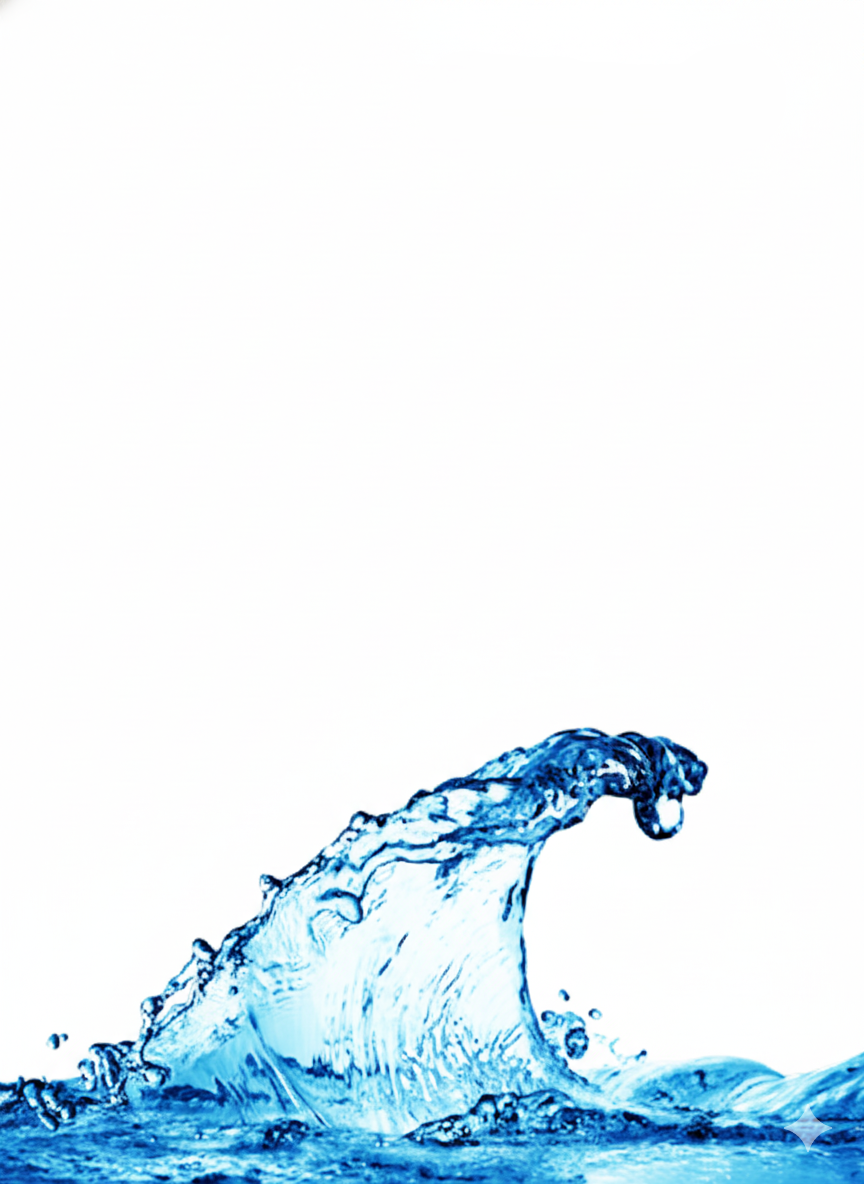
\includegraphics[width=\paperwidth, height=\paperheight]{fond.png}
    };
\end{tikzpicture}



\begin{center}

\textsc{\Large{Preuve de concept}}
\HRule
\vspace*{0.1cm}
\textsc{\huge{\textbf{Optimisation de trajectoire par B-Spline\\}}}
\vspace*{0.2cm}
\textsc{\huge{\textbf{Initialement pour le Robot Club Toulon}}}
\HRule
\vspace*{0.5cm}
\large{SeaTech, Toulon, France\\} 
\vspace*{0.2cm}
\large{Décembre 2025 - Octobre 2026 \\} 
\vspace*{0.2cm}
\large{Timm Claverie\\}



\end{center}
\end{titlepage}
\ClearShipoutPicture

\tableofcontents
\thispagestyle{empty}
\newpage

% ==============================================================================
% RESUME + MOTS CLES
% ==============================================================================

\begin{abstract}

Ce rapport présente une chaîne hybride de trajectographie pour robots mobiles, combinant courbes de Bézier cubiques, apprentissage supervisé et raffinement cinématique. Un dataset de trajectoires optimales est d’abord généré hors-ligne sous contraintes de vitesse et d’accélération, puis un réseau de neurones ultra-léger est entraîné pour prédire le temps optimal de parcours. L’inférence est sécurisée par un ajustement analytique garantissant le respect des limites \(V_{\max}\) et \(A_{\max}\). L’approche, validée en 2D puis étendue en 3D, permet une exécution temps réel compatible avec une boucle à \(50\)~Hz. Initialement destiné à un robot footballer au sol, le système est appliqué à un drone en vol et ouvre la voie à des missions embarquées à vitesse d’arrivée contrôlée.\\

Mots clés : \textit{trajectographie}, \textit{courbes de Bézier}, \textit{apprentissage supervisé}, \textit{contrôle cinématique}, \textit{temps réel}, \textit{drone}, \textit{robot mobile}

\end{abstract}


% ==============================================================================
% INTRODUCTION
% ==============================================================================
\chapter{Introduction}

Ce rapport présente la conception d’un contrôleur de trajectoire pour robots mobiles combinant apprentissage supervisé et contraintes cinématiques. L’objectif est de remplacer les solveurs de planification lourds par une chaîne hybride légère : un réseau de neurones estime le temps optimal \(T_{opt}\) d’un déplacement entre deux points, puis un raffinement analytique garantit le respect strict des vitesses et accélérations maximales \(V_{\max}\) et \(A_{\max}\).\\

La démarche s’articule en trois étapes : génération hors-ligne d’un dataset de trajectoires de Bézier cubiques contraintes par les vitesses de départ et d’arrivée, entraînement d’un réseau ultra-léger, puis inférence embarquée avec correction physique. L’architecture est d’abord validée en 2D, avant d’être étendue en 3D via une base locale orthonormée.

\begin{figure}[H]
\centering

\includegraphics[width=6cm]{rct.png}
\end{figure}

Initialement destiné à un robot footballer au sol pour le Robot Club Toulon (RCT), le système est ensuite adapté à un drone évoluant en volume 3D. Les résultats montrent une exécution compatible avec une boucle à \(50\)~Hz, ouvrant la voie à des applications embarquées telles que l’évitement d’obstacles ou l’interception à vitesse contrôlée.




% ==============================================================================
% CHAPITRE 1 : GENERATION (VERSION DÉTAILLÉE)
% ==============================================================================
\chapter{Phase 1 : Génération du Dataset et Modélisation}
\label{chap:generation}

Cette première phase est critique : elle constitue la "Vérité Terrain" (\textit{Ground Truth}) nécessaire à l'apprentissage supervisé. Le script \texttt{generateur.py} utilise une approche inverse : il détermine analytiquement la trajectoire géométrique idéale pour satisfaire des contraintes cinématiques temporelles.

\section{Fondements Théoriques : B-Splines et Courbes de Bézier}

\subsection{Définition et Distinction}
Dans la planification de trajectoire, nous cherchons à définir une courbe paramétrique continue $C(u)$. Deux familles mathématiques sont couramment utilisées : les B-Splines et les courbes de Bézier.

\begin{itemize}
    \item \textbf{B-Splines (Basis Splines) :} Ce sont des fonctions définies par morceaux, offrant un contrôle local. Modifier un point de contrôle n'affecte qu'une partie de la courbe. Elles sont idéales pour des trajectoires longues et complexes traversant de multiples points de passage (waypoints).
    \item \textbf{Courbes de Bézier :} C'est un cas particulier de B-Splines. Une courbe de Bézier de degré $n$ est définie par $n+1$ points de contrôle. Contrairement aux B-Splines générales, une courbe de Bézier passe \textbf{toujours} par son premier ($P_0$) et son dernier point ($P_n$), ce qui est impératif pour notre problème (départ et arrivée précis du robot).
\end{itemize}

Dans le cadre de ce projet, le script utilise des \textbf{Courbes de Bézier Cubiques} (degré 3). Ce choix offre le compromis optimal : assez de degrés de liberté pour définir la position et la tangence (vitesse) aux deux extrémités, sans la complexité de calcul des B-Splines de degré supérieur.

\subsection{Équation Canonique}
Une courbe de Bézier cubique est définie pour un paramètre adimensionnel $u \in [0, 1]$ par :

\begin{equation}
    B(u) = (1-u)^3 P_0 + 3(1-u)^2 u P_1 + 3(1-u) u^2 P_2 + u^3 P_3
\end{equation}

Où :
\begin{itemize}
    \item $P_0$ : Position de départ (Robot).
    \item $P_3$ : Position d'arrivée (Cible).
    \item $P_1, P_2$ : Points de contrôle influençant la tangente et la courbure.
\end{itemize}

\section{Couplage Géométrie-Cinématique}

Le calcul des points $P_1$ et $P_2$, habituellement fixés arbitrairement, sont ici calculés pour respecter scrupuleusement les vitesses $v_{start}$ et $v_{end}$.

\subsection{Démonstration}
Pour comprendre les formules utilisées dans le code, il faut dériver l'équation de Bézier par rapport au temps $t$.
Soit $T$ la durée totale du mouvement. On a la relation $u = \frac{t}{T}$, donc $\frac{du}{dt} = \frac{1}{T}$.

La vitesse vectorielle $\vec{V}(t)$ est la dérivée temporelle de la position :
\begin{equation}
    \vec{V}(t) = \frac{dB(u)}{du} \cdot \frac{du}{dt} = \frac{dB(u)}{du} \cdot \frac{1}{T}
\end{equation}

Calculons la dérivée par rapport à $u$ à l'origine ($u=0$, soit le départ) :
\begin{align*}
    \frac{dB}{du}(0) &= \lim_{u \to 0} \frac{d}{du} \left[ (1-u)^3 P_0 + 3(1-u)^2 u P_1 + \dots \right] \\
    &= 3(P_1 - P_0)
\end{align*}

En réinjectant dans l'équation de vitesse au temps $t=0$ :
\begin{equation}
    \vec{V}_{start} = 3(P_1 - P_0) \cdot \frac{1}{T}
\end{equation}

Si l'on isole $P_1$, on obtient la formule utilisée dans le code :
\begin{equation}
    P_1 = P_0 + \frac{\vec{V}_{start} \cdot T}{3}
\end{equation}

En notant $\vec{V}_{start} = v_{start} \cdot \vec{u}_{start}$ (norme $\times$ direction), on retrouve exactement l'implémentation Python. Le facteur $3$ provient donc directement du degré du polynôme cubique.


\subsection{Calcul du point de contrôle $P_2$ (Arrivée)}

Le point $P_2$ joue un rôle symétrique à $P_1$ : il conditionne l'approche finale vers la cible $P_3$. Il permet de définir l'angle d'arrivée (tangente) et la vitesse finale instantanée ($v_{end}$).

\subsubsection{Dérivation Mathématique}
Tout comme pour le départ, nous partons de la dérivée de la courbe de Bézier par rapport au paramètre $u$, mais cette fois-ci évaluée à la fin de la trajectoire, c'est-à-dire en $u=1$.

La dérivée d'une courbe de Bézier cubique en $u=1$ est déterminée par le vecteur formé par les deux derniers points de contrôle :
\begin{equation}
    \frac{dB}{du}(1) = 3(P_3 - P_2)
\end{equation}

En appliquant la règle de la chaîne pour passer du domaine géométrique ($u$) au domaine temporel ($t$), avec $\vec{V}(t) = \frac{dB}{du} \cdot \frac{1}{T}$, nous obtenons la vitesse à l'instant final $t=T$ :

\begin{equation}
    \vec{V}_{end} = \frac{1}{T} \cdot 3(P_3 - P_2)
\end{equation}

Notre objectif est d'isoler $P_2$. En manipulant l'équation :
\begin{align*}
    T \cdot \vec{V}_{end} &= 3(P_3 - P_2) \\
    \frac{T \cdot \vec{V}_{end}}{3} &= P_3 - P_2 \\
    P_2 &= P_3 - \frac{T \cdot \vec{V}_{end}}{3}
\end{align*}

\subsubsection{Interprétation Géométrique et Code}
L'équation finale révèle une différence fondamentale avec $P_1$ : la présence du signe \textbf{moins}.

Géométriquement, cela s'explique simplement : le vecteur vitesse $\vec{V}_{end}$ pointe vers "l'avant" (la direction du mouvement à l'arrivée). Or, le point $P_2$ est situé \textit{avant} $P_3$ dans le temps. Pour trouver $P_2$ à partir de la cible $P_3$, il faut donc "reculer" le long de la tangente.

Dans le script \texttt{generateur.py}, cette logique est implémentée explicitement :

\begin{lstlisting}[language=Python, caption={Calcul "Rétrograde" de P2}]
# u_end : Vecteur unitaire de direction a l'arrivee
u_end = np.array([np.cos(theta_end), np.sin(theta_end)])

# Distance de recul proportionnelle a la vitesse et au temps
dist_tan_end = (v_end * T) / 3.0

# On part de la cible (P3) et on soustrait le vecteur
P2 = P3 - dist_tan_end * u_end
\end{lstlisting}

Cette formulation garantit que si le robot doit arriver avec une vitesse élevée ($v_{end}$ grand), $P_2$ sera placé loin en arrière de $P_3$, forçant la trajectoire à s'aligner progressivement bien avant l'arrivée. À l'inverse, si $v_{end}=0$ (arrêt au stand), alors $P_2 = P_3$, ce qui géométriquement écrase la fin de la courbe pour forcer une décélération.


\subsection{Implémentation Algorithmique}
Le code traduit cette contrainte mathématique dans la fonction \texttt{get\_control\_points\_from\_velocity} :

\begin{lstlisting}[language=Python, caption={Calcul des points de contrôle sous contrainte}]
def get_control_points_from_velocity(P0, P3, theta_start, theta_end, v_start, v_end, T):
    # Vecteurs unitaires de direction
    u_start = np.array([np.cos(theta_start), np.sin(theta_start)])
    u_end   = np.array([np.cos(theta_end), np.sin(theta_end)])
    
    # Application de la formule derivee ci-dessus
    # V(0) = 3(P1-P0)/T  =>  dist = v * T / 3
    dist_tan_start = (v_start * T) / 3.0
    dist_tan_end   = (v_end * T) / 3.0
    
    P1 = P0 + dist_tan_start * u_start
    P2 = P3 - dist_tan_end * u_end
    
    return P1, P2
\end{lstlisting}






\section{Le Solveur Temporel (Time Optimal Solver)}

Une fois la géométrie liée au temps $T$ par les formules ci-dessus, il reste une inconnue : \textbf{Quel est le temps $T$ minimal réalisable ?}

Si $T$ est trop court, la distance $P_0 \rightarrow P_1$ devient très petite (car proportionnelle à $T$), mais la vitesse demandée reste la même, ce qui implique une accélération mathématiquement nécessaire qui peut dépasser les capacités du moteur.

Le script utilise une approche de \textbf{Recherche Dichotomique} (bisection) pour trouver ce $T$ :

\begin{enumerate}
    \item Tolérance de 5 ms pour trouver le T minimal faisable
    \item Pour chaque candidat $T_{test}$ :
    \begin{itemize}
        \item On calcule $P_1$ et $P_2$ avec les formules de vitesse.
        \item On échantillonne la courbe (25 points).
        \item On calcule l'accélération en tout point : $\vec{A}(t) = \frac{d^2B}{dt^2}$.
    \end{itemize}
    \item Si $\max(||\vec{A}(t)||) \leq A_{max\_robot}$ et $\max(||\vec{V}(t)||) \leq V_{max\_robot}$, alors $T_{test}$ est valide.
    \item Le premier $T$ valide trouvé est conservé comme $T_{opt}$.
\end{enumerate}

C'est cette valeur $T_{opt}$, issue d'une simulation physique complexe, qui servira d'étiquette (Label) pour entraîner le réseau de neurones dans la phase suivante.
















% ==============================================================================
% CHAPITRE 2 : APPRENTISSAGE
% ==============================================================================
\chapter{Phase 2 : Apprentissage Supervisé}

Le script \texttt{entrainement.py} charge le dataset généré pour entraîner un modèle de régression léger.

\section{Architecture du Modèle}
Le réseau de neurones, nommé \texttt{TimePredictorNet}, est un Perceptron Multi-Couches (MLP) conçu pour l'inférence rapide. Le modèle $6 \rightarrow 18 \rightarrow 5 \rightarrow 1 $  (environ $250$ paramètres). Cette légèreté permet une inférence en $0.07$ ms. 

\begin{itemize}
    \item \textbf{Entrée (6 neurones) :} $x_{local}, y_{local}, \cos\theta_{target}, \sin\theta_{target}, v_{start}, v_{end}$.
    \item \textbf{Couches Cachées :} 
        \begin{itemize}
            \item Linear(18) + ReLU
            \item Linear(5) + ReLU
        \end{itemize}
    \item \textbf{Sortie (1 neurone) :} Temps Optimal $T$.
\end{itemize}

\begin{figure}[h]
\centering
\begin{tikzpicture}[x=1.5cm, y=1.2cm, >=stealth]
    % Input Layer
    \foreach \m [count=\y] in {1,2,3,4}
      \node [circle, draw, fill=green!20, minimum size=0.8cm] (I-\m) at (0,2.5-\y) {};
    \node at (0, 2.5) {Input};
    
    % Hidden Layer
    \foreach \m [count=\y] in {1,2,3,4,5}
      \node [circle, draw, fill=blue!20, minimum size=0.8cm] (H-\m) at (2,3-\y) {};
    \node at (2, 3) {Hidden};
    
    % Output Layer
    \node [circle, draw, fill=red!20, minimum size=0.8cm] (O) at (4,0) {$T$};
    \node at (4, 1) {Output};

    % Connections (Simplified)
    \foreach \i in {1,...,4}
      \foreach \j in {1,...,5}
        \draw [->, gray!50] (I-\i) -- (H-\j);
    
    \foreach \j in {1,...,5}
      \draw [->, gray!50] (H-\j) -- (O);
\end{tikzpicture}
\caption{Exemple de schéma simplifié d'une architecture neuronale}
\end{figure}

\section{Normalisation et Reconstruction}
Un point critique relevé dans le code est la normalisation des données (Z-Score normalization). Les statistiques ($mean, std$) sont sauvegardées dans \texttt{statistique\_de\_normalisation.npz} car elles sont indispensables pour l'inférence.

Le modèle ne prédit que le temps. La géométrie de la courbe est reconstruite géométriquement après la prédiction, garantissant ainsi que la trajectoire reste mathématiquement une courbe de Bézier valide, même si la prédiction du temps comporte une légère erreur.

\section{Stratégie Hybride IA + Physique}
L'IA fournit une estimation initiale très rapide ("Initial Guess"). Cependant, pour garantir la sécurité du robot, cette estimation est raffinée par un algorithme d'optimisation local.

Le processus se déroule comme suit :
\begin{enumerate}
    \item \textbf{Prédiction :} Le modèle estime $T_{pred}$.
    \item \textbf{Audit :} On calcule les pics d'accélération et de vitesse pour ce $T_{pred}$.
    \item \textbf{Correction :} Si les contraintes sont violées (ratio $> 1$), on augmente $T$. Si le robot est en sous-régime, on diminue $T$.
\end{enumerate}

La prédiction du réseau est raffinée par une bisection stricte sur les contraintes physiques (marge de sécurité de $1\%$ sur Vmax et Amax). Cela garantit mathématiquement une trajectoire réalisable, sans dépassement, en un temps borné (maximum $40$ itérations).








% ==============================================================================
% CHAPITRE 5 - À INSÉRER DANS TON DOCUMENT PRINCIPAL
% (Remplace \section par \chapter si ton document utilise la classe report/book)
% ==============================================================================

\chapter{Extension au cas 2D et Validation Temps Réel}
\label{sec:poc_2d}

Ce chapitre présente l'évolution du système vers un POC complet pour la robotique 2D. L'objectif est de générer des trajectoires en 360°, de garantir le respect strict des contraintes cinématiques, et de valider une exécution à 50 Hz sur CPU.

\section{Génération du Dataset : Couverture 360° et Solveur Exact}

La version précédente générait uniquement des cibles situées devant le robot (angle restreint). Pour un POC robuste, le dataset a été régénéré avec une couverture totale de 360° (cibles devant et derrière le robot). 

Le solveur temporel a également été amélioré. Au lieu d'un balayage linéaire, le script \texttt{generateur.py} utilise une \textbf{recherche par dichotomie} pour trouver le $T_{opt}$ quasi-optimal sous tolérance respectant \(V_{max}=6.5\) m/s et \(A_{max}=6.0\) m/s\(^2\). 

\begin{figure}[H]
    \centering
    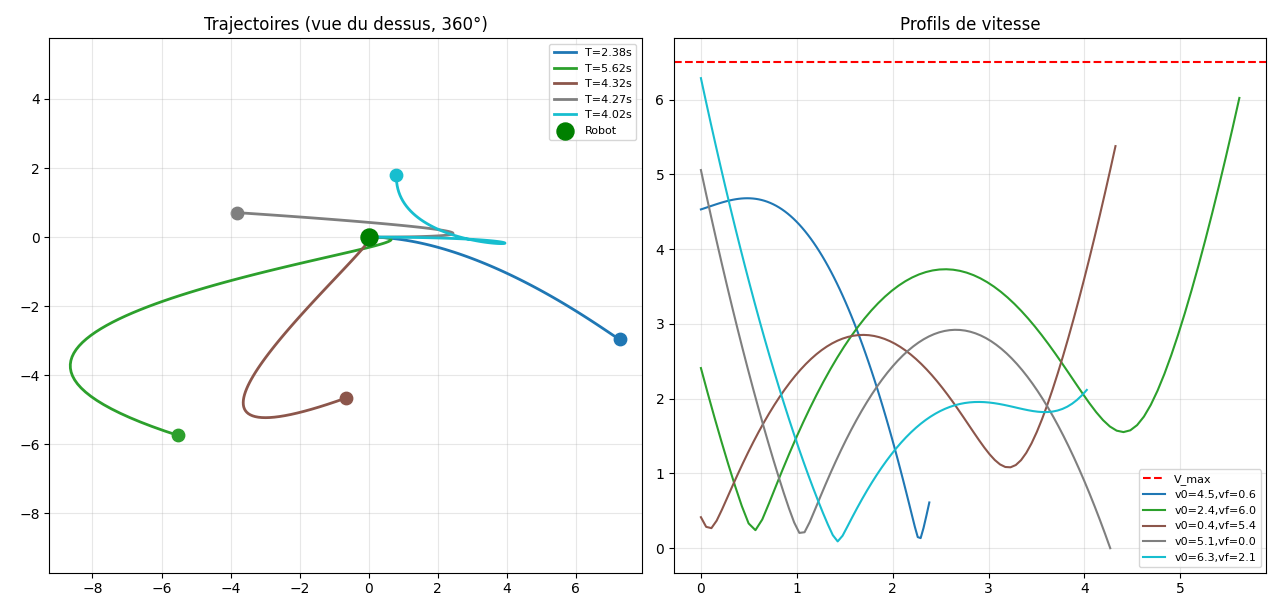
\includegraphics[width=0.95\textwidth]{generation.png}
    \caption{Trajectoires générées en 360° et profils de vitesse associés. On observe que les cas nécessitant un demi-tour génèrent des trajectoires plus longues et des temps $T$ plus élevés, respectant scrupuleusement les limites physiques.}
    \label{fig:dataset_360}
\end{figure}

\begin{itemize}
    \item \textbf{Dataset final} : 20 000 échantillons.
    \item \textbf{Temps optimal ($T_{opt}$)} : varie de 0.8 s à 8.5 s selon la distance et le profil de vitesse.
\end{itemize}

\section{Apprentissage Supervisé : Un Réseau Neuronal Ultra-Léger}

Pour garantir l'exécution sur un processeur standard (CPU) sans GPU, le réseau \texttt{TimePredictorNet} a été réduit à sa plus simple expression tout en conservant sa capacité de prédiction. Il ne prédit qu'une seule valeur : le temps optimal $T_{opt}$.

\begin{itemize}
    \item \textbf{Entrées (6)} : $x_{local}$, $y_{local}$, $\cos(\theta)$, $\sin(\theta)$, $v_{start}$, $v_{end}$.
    \item \textbf{Couches} : \texttt{Linear(6, 18)} \(\rightarrow\) ReLU \(\rightarrow\) \texttt{Linear(18, 5)} \(\rightarrow\) ReLU \(\rightarrow\) \texttt{Linear(5, 1)}.
    \item \textbf{Paramètres} : \(\approx 250\) poids.
\end{itemize}

L'entraînement (80\% Train / 20\% Validation) a été effectué sur 300 époques avec un scheduler réduisant le learning rate si la validation stagne.

\begin{figure}[H]
    \centering
    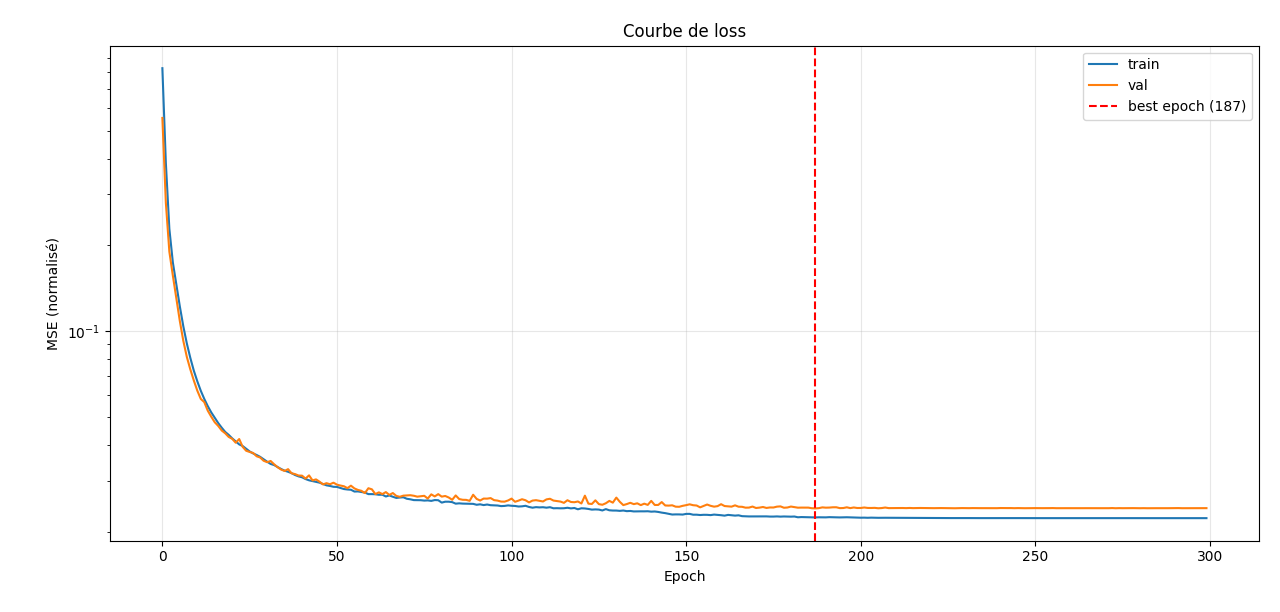
\includegraphics[width=0.8\textwidth]{entrainement.png} % À remplacer par le nom de ton image
    \caption{Courbe d'apprentissage. Le modèle converge rapidement dès l'époque 50, et le meilleur modèle (\textit{Early Stopping}) est atteint à l'époque 187. L'écart train/val est minime, prouvant l'absence de surapprentissage.}
    \label{fig:loss_curve}
\end{figure}

\section{Contrôleur Hybride et Exécution 50 Hz}

L'inférence pure du réseau neuronal (0.07 ms) est couplée à un module physique \texttt{refine\_time\_with\_physics}. Ce module utilise une \textbf{dichotomie} pour s'assurer que les points de contrôle Bézier respectent à 99\% les limites du robot (marge de sécurité de 1\%).

Pour valider le POC, un exécuteur (\texttt{TrajectoryExecutor}) a été implémenté avec deux modes :
\begin{enumerate}
    \item \textbf{Mode CACHED} : Le plan est calculé une fois, on ne fait qu'échantillonner la courbe.
    \item \textbf{Mode REPLAN} : On recalcule le plan à chaque pas de temps (simulation de cibles mouvantes ou d'évitement d'obstacles dynamique).
\end{enumerate}

\begin{figure}[H]
    \centering
    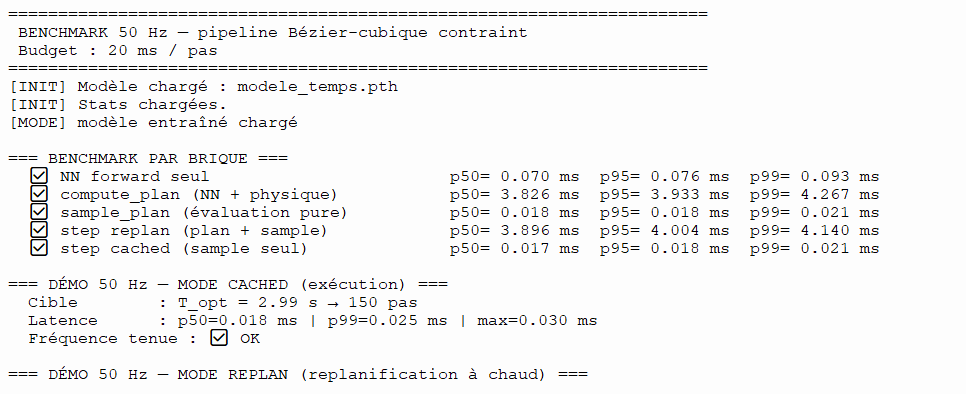
\includegraphics[width=\textwidth]{benchmark.png} % À remplacer par le nom de ton image
    \caption{Benchmark de latence. Le mode "cached" s'exécute en 0.018 ms. Le mode "replanification" complet (NN + Physique + Bézier) s'exécute en p99=4.14 ms. Les deux modes respectent largement le budget de 20 ms par pas pour une boucle à 50 Hz.}
    \label{fig:benchmark}
\end{figure}

\section{Résultats Visuels et Analyse Cinématique}

Le scénario de test le plus critique est celui où la cible est située \textbf{derrière} le robot, avec un changement d'orientation (ex: robot en \((0,0)\) vers la cible en \((-2,-1)\)). Ce cas force le robot à effectuer un virage très serré.

\begin{figure}[H]
    \centering
    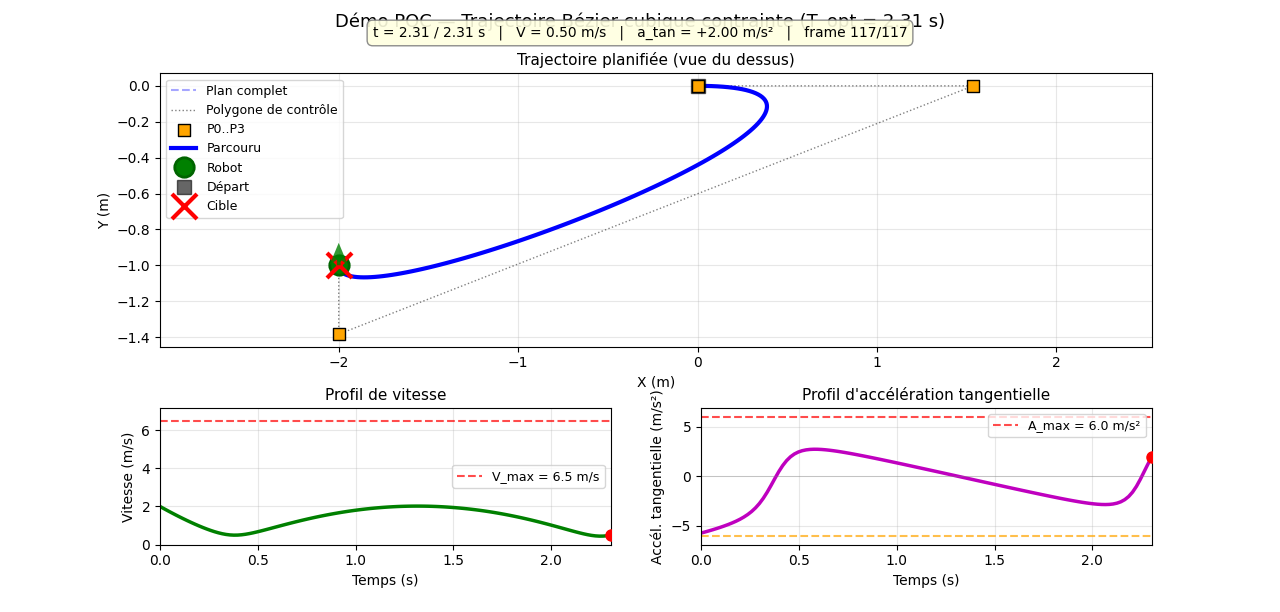
\includegraphics[width=\textwidth]{demo.png} % À remplacer par le nom de ton image
    \caption{Démo de la trajectoire vers \((-2,-1)\). Le robot ralentit fortement au milieu de la courbe pour respecter la force centrifuge. À l'arrivée, l'accélération tangentielle atteint exactement la limite de freinage (\(-6.0\) m/s\(^2\)), validant le respect strict des contraintes physiques.}
    \label{fig:demo_trajectoire}
\end{figure}

\begin{itemize}
    \item \textbf{Analyse de la trajectoire} : Le profil de vitesse montre une décélération de \(2.0\) m/s à \(0.5\) m/s pour passer le virage, puis une ré-accélération. 
    \item \textbf{Respect des contraintes} : Le profil d'accélération tangentielle sature exactement à \(+6.0\) et \(-6.0\) m/s\(^2\), prouvant que le solveur physique extrait le maximum des capacités du robot (\textit{time-optimal}).
    \item \textbf{Embarqué} : Le réseau de neurones fournit le $T_{opt}$ en une fraction de milliseconde, permettant de recalculer cette trajectoire complexe 50 fois par seconde si nécessaire.
\end{itemize}

\section{Conclusion du POC}

Ce POC démontre qu'il est possible de remplacer un solveur d'optimisation non-linéaire lourd par un réseau de neurones de 250 paramètres, tout en garantissant la sécurité cinématique via un raffinement analytique. L'architecture est prête pour être déployée sur un microcontrôleur ou un Raspberry Pi pour du contrôle temps réel.






% ==============================================================================
% CHAPITRE 6 - EXTENSION AU CAS 3D
% ==============================================================================

\chapter{Extension au cas 3D}
\label{sec:poc_3d}

Ce chapitre présente l'adaptation du système pour la navigation en volume 3D. L'architecture globale (réseau ultra-léger, reconstruction analytique et raffinement physique) reste identique à la version 2D. Les différences résident dans la gestion du repère local et dans les dimensions des tenseurs d'entrée.

\section{Génération du Dataset : Repère Local 3D}

La difficulté majeure du passage en 3D est le changement de repère. En 2D, une simple rotation d'angle \(\theta\) suffisait. En 3D, le robot évolue dans un espace où sa direction est un vecteur tridimensionnel. 

Pour que le réseau de neurones puisse apprendre efficacement, le problème doit être invariant par rotation. Nous construisons donc une \textbf{base orthonormée locale} \((\vec{u}, \vec{v}, \vec{w})\) attachée au robot :
\begin{itemize}
    \item \(\vec{u}\) : Vecteur directeur du robot (normalisé).
    \item \(\vec{v}\) : Vecteur orthogonal à \(\vec{u}\) (généré par produit vectoriel avec l'axe \(Z\) global, ou l'axe \(Y\) si \(\vec{u}\) est colinéaire à \(Z\)).
    \item \(\vec{w}\) : Vecteur orthogonal complétant la base (\(\vec{w} = \vec{u} \wedge \vec{v}\)).
\end{itemize}

La matrice de passage \(R\) (de taille \(3 \times 3\)) permet de projeter la cible dans le repère local du robot :
\[ \vec{P}_{local} = R \cdot (\vec{P}_{cible} - \vec{P}_{robot}) \]
La cible est ainsi générée aléatoirement dans une sphère complète (coordonnées sphériques) et son vecteur d'arrivée est également projeté. Le dataset résultant contient 8 entrées au lieu de 6 : \((x_{loc}, y_{loc}, z_{loc}, u_x, u_y, u_z, v_{start}, v_{end})\).

Le solveur temporel (dichotomie) reste inchangé, mais les normes de vitesse et d'accélération sont calculées en 3D : \(\|\vec{V}\| = \sqrt{v_x^2 + v_y^2 + v_z^2}\).

\section{Apprentissage Supervisé}

L'architecture du réseau \texttt{TimePredictorNet} a été légèrement élargie pour absorber la dimension supplémentaire :
\begin{itemize}
    \item \textbf{Entrées (8)} : \(x_{loc}\), \(y_{loc}\), \(z_{loc}\), \(u_x\), \(u_y\), \(u_z\), \(v_{start}\), \(v_{end}\).
    \item \textbf{Couches} : \texttt{Linear(8, 20)} \(\rightarrow\) ReLU \(\rightarrow\) \texttt{Linear(20, 10)} \(\rightarrow\) ReLU \(\rightarrow\) \texttt{Linear(10, 1)}.
    \item \textbf{Paramètres} : \(\approx 400\) poids.
\end{itemize}
La cible d'apprentissage reste le temps optimal \(T_{opt}\). La reconstruction des points de contrôle de Bézier s'effectue ensuite de manière déterministe dans le repère local, avant d'être ramenée dans le repère global via la transposée de la matrice \(R\).

\section{Contrôleur Hybride et Exécution 50 Hz}

Le contrôleur physique \texttt{refine\_time\_with\_physics} vérifie les contraintes sur la courbe 3D. Pour valider les performances, le benchmark mesure les mêmes briques d'exécution.

\begin{figure}[H]
    \centering
    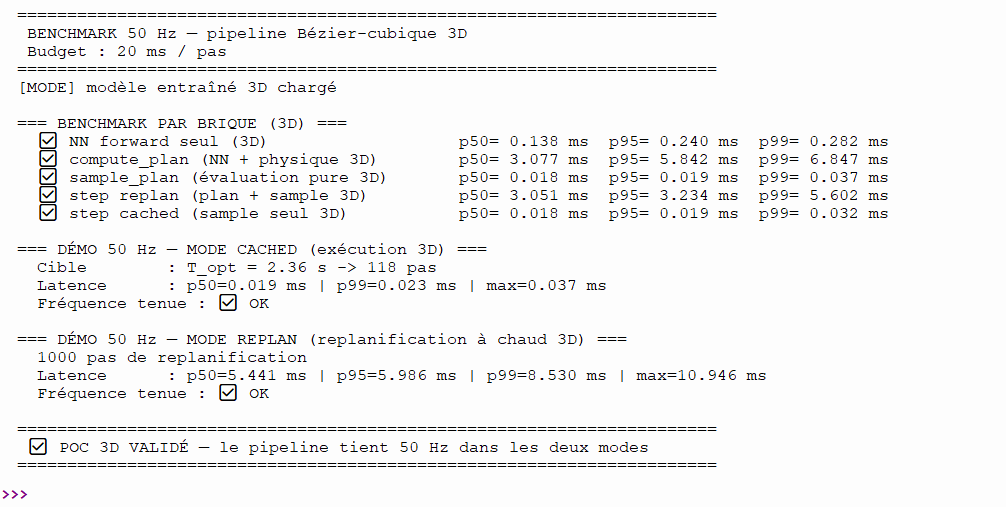
\includegraphics[width=\textwidth]{benchmark2.png}
    \caption{Benchmark de latence pour le pipeline 3D. Le calcul complet d'un plan (NN + Physique) s'exécute en \(p99 = 6.8\) ms. Le mode "replanification à chaud" (simulant un mouvement continu du robot) prend au maximum \(10.9\) ms par cycle. Les deux modes respectent largement le budget de 20 ms pour une boucle à 50 Hz.}
    \label{fig:benchmark_3d}
\end{figure}

\section{Résultats Visuels et Analyse Cinématique}

Ce scénario de test illustre un déplacement avec un fort changement d'élévation. Le robot part de l'origine vers une cible en hauteur, nécessitant une courbure 3D.

\begin{figure}[H]
    \centering
    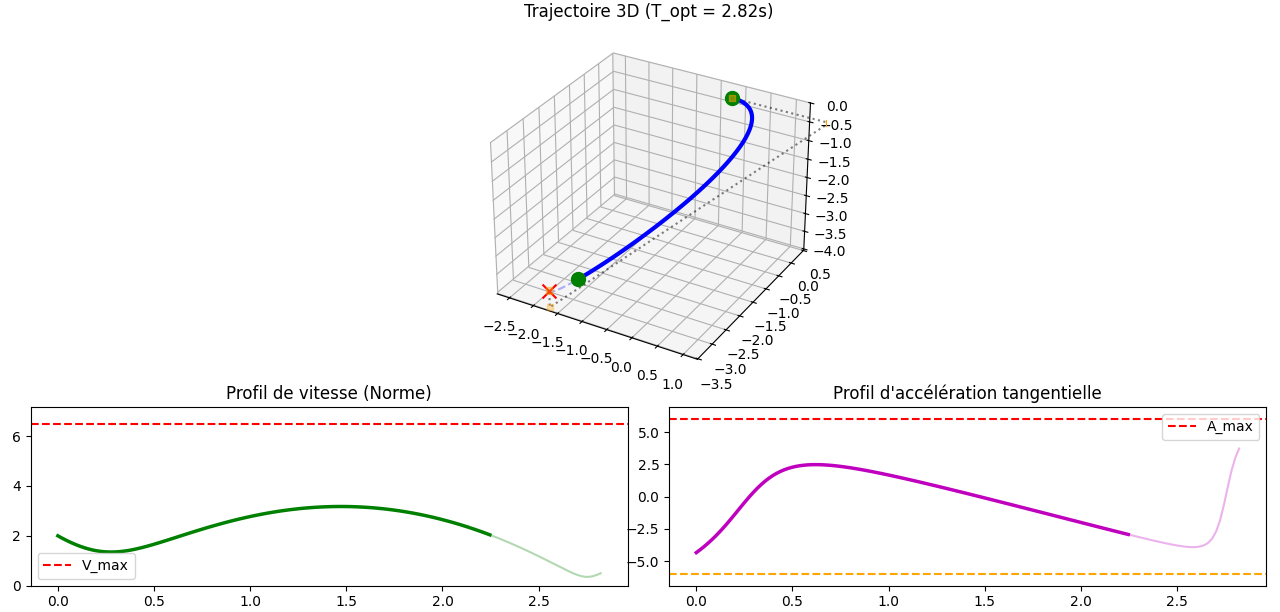
\includegraphics[width=\textwidth]{demo2.png}
    \caption{Démonstration de la trajectoire 3D. En haut : la trajectoire dans le volume (courbe bleue). En bas : les profils de vitesse et d'accélération tangentielle. Les limites \(V_{max}\) et \(A_{max}\) sont parfaitement respectées, démontrant l'efficacité du raffinement physique dans l'espace 3D.}
    \label{fig:demo_3d}
\end{figure}

\begin{itemize}
    \item \textbf{Analyse de la trajectoire} : La norme de la vitesse (graphique en bas à gauche) montre une accélération franche pour sortir de l'axe initial, suivie d'une phase de croisière. Le profil d'accélération tangentielle sature à \(+6.0\) et \(-6.0\) m/s\(^2\).
    \item \textbf{Embarqué} : La légèreté du réseau (400 poids) permet d'effectuer cette planification 3D en moins de \(7\) ms, ouvrant la voie à des applications de drones ou de bras manipulateurs temps réel.
\end{itemize}

\section{Conclusion du POC 3D}

L'extension en 3D démontre la robustesse de l'architecture hybride. Le passage d'un problème 2D à un problème 3D ne nécessite qu'une adaptation de la base locale (matrice de rotation) et une légère modification du réseau. Le cœur du système (recherche de \(T_{opt}\) et reconstruction de Bézier) reste identique et garantit une exécution temps réel sans explosion combinatoire.





\chapter{Système de trajectographie 3D pour drone}

Ce chapitre illustre, au travers d'une simulation, un cas où un drone en vol 
reçoit des consignes de déplacement dans un environnement 3D. On suppose que 
le système de décision du drone fournit à notre modèle de trajectoire des 
waypoints exprimés dans le repère local du drone, de la forme 
$[x, y, z, dir_x, dir_y, dir_z, vitesse]$ : $(x, y, z)$ désigne la position 
relative de la cible, $(dir_x, dir_y, dir_z)$ la direction d'arrivée 
souhaitée, et $vitesse$ la vitesse de passage au waypoint.

Travailler dans un repère relatif présente deux intérêts majeurs. D'une part,
le calcul du point visé ne dépend plus d'un repère absolu : le modèle est donc
plus robuste aux dérives de localisation, et la nécessité d'un SLAM est
supprimée. D'autre part, la consigne transmise au modèle est directement
exploitable par le contrôleur bas niveau du drone, sans étape de
transformation intermédiaire.

Le drone ne contrôle pas l'intégralité de sa trajectoire à l'avance : si un
obstacle apparaît sur la trajectoire planifiée, le recalcul complet — qui
s'effectue à moins de $20$~Hz — permet d'insérer de nouveaux waypoints afin
de contourner l'obstacle, tout en préservant la continuité de vitesse et de
cap.

\begin{figure}[H]
    \centering
    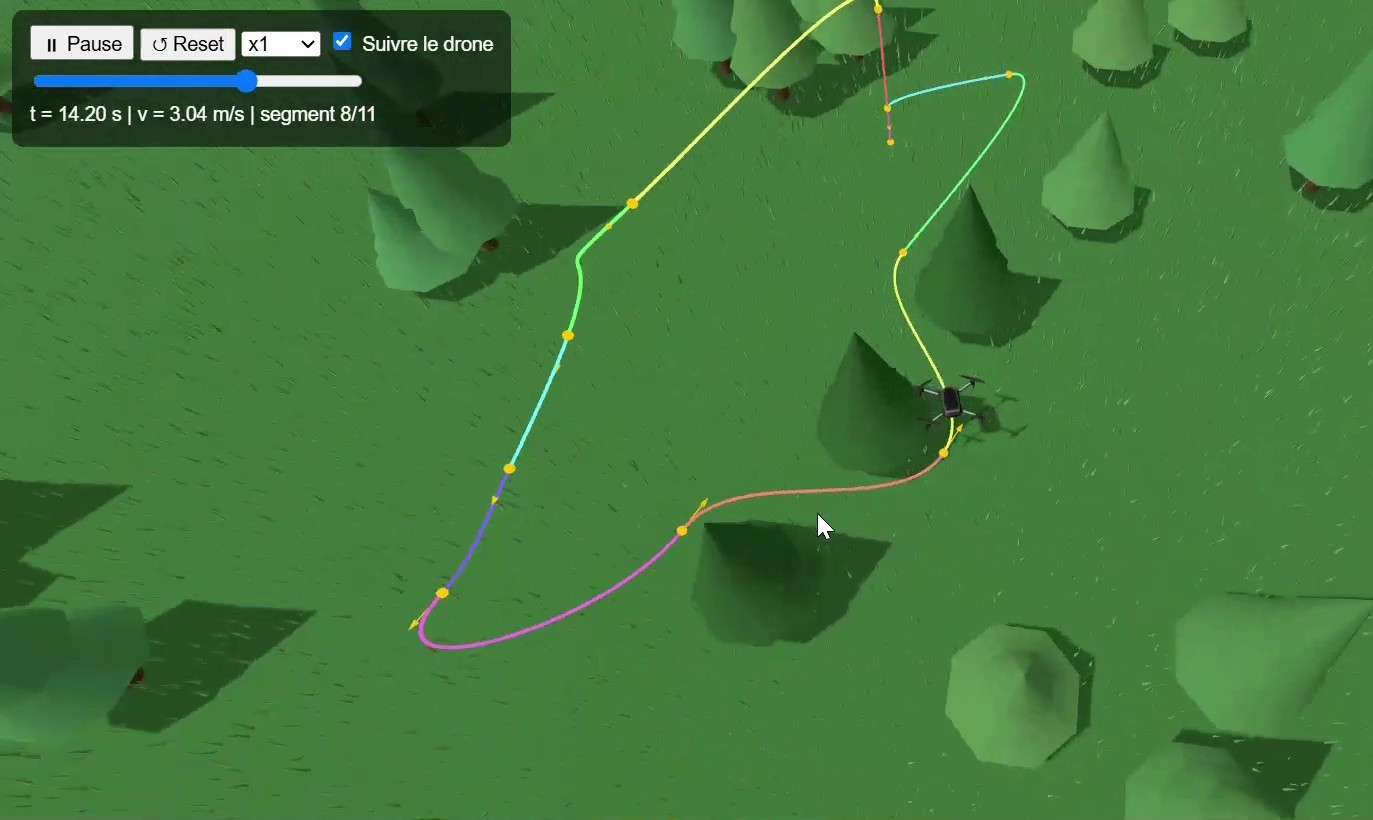
\includegraphics[width=\textwidth]{simufinal.jpg}
    \caption{Démonstration d'une trajectoire 3D calculée par le modèle, avec un
    drone évoluant en forêt et évitant les arbres.}
    \label{fig:demo_3d}
\end{figure}

Les principaux avantages du modèle sont :
\begin{enumerate}
    \item un calcul de trajectoire en environ $10$~ms, compatible avec une
          replanification à $50$~Hz ;
    \item la possibilité d'imposer la vitesse d'arrivée au passage de chaque
          waypoint.
\end{enumerate}










\chapter{Conclusion}

Ce rapport a présenté une chaîne complète de génération, d’apprentissage et d’exécution de trajectoires pour robots mobiles. En résumé, la démarche repose sur trois étapes : (i) la génération hors-ligne d’un dataset de trajectoires optimales à partir de courbes de Bézier cubiques contraintes par les vitesses de départ et d’arrivée, (ii) l’entraînement d’un réseau de neurones ultra-léger prédisant le temps optimal \(T_{opt}\), et (iii) une exécution hybride où l’inférence neuronale est sécurisée par un raffinement analytique des contraintes cinématiques \(V_{\max}\) et \(A_{\max}\). L’architecture a d’abord été validée en 2D, puis étendue en 3D via une base locale orthonormée et une matrice de rotation. Les benchmarks montrent que le pipeline respecte largement le budget temps réel : inférence du réseau en environ \(0.07\)~ms, calcul complet d’un plan 3D en quelques millisecondes, et replanification à chaud compatible avec une boucle à \(\sim50 \)Hz, soit un budget de \(20\)~ms par pas. La démonstration en environnement 3D, avec un drone évoluant en forêt et contournant des arbres, illustre le bon fonctionnement global du système.\\

L’objectif initial de ce travail était de concevoir un système de trajectographie pour un robot footballer au sol, capable de rejoindre un waypoint avec une vitesse de départ, une vitesse d’arrivée et une direction imposées, tout en minimisant le temps de parcours et en respectant les limites physiques du robot. Ce cadre a ensuite été étendu à un système 3D pour drone. Le passage en 3D ne remet pas en cause l’architecture : il nécessite principalement une adaptation du repère local, une projection de la cible dans ce repère et un élargissement léger du réseau de neurones. Le cœur du système — prédiction du temps optimal, reconstruction géométrique de la courbe de Bézier et raffinement physique — reste identique.\\

Enfin, la légèreté du modèle neuronal, environ \(400\) poids dans sa version 3D, et sa très faible latence d’inférence permettent d’envisager son embarquement sur un drone à impact, également appelé drone kamikaze ou munition rôdeuse. Dans ce contexte, le modèle peut planifier une trajectoire relative vers une cible et imposer une vitesse d’arrivée ainsi qu’une direction d’impact précises, tout en respectant les contraintes de vitesse et d’accélération maximales. La capacité de replanification à \(50\)~Hz offre de plus une marge intéressante pour l’évitement d’obstacles ou l’adaptation à une cible mobile. Ce travail ouvre donc la voie à des perspectives d’embarquement réel, de validation sur drone physique et d’extension à des missions d’interception ou d’assaut terminal à vitesse contrôlée.




\end{document}